\chapter{Background}
\label{chap:background}

\section{Introduction}

This chapter provides an overview of the techniques and theory used in this thesis. Sections~\ref{sec:background-machine-learning} and~\ref{sec:evaluation-techniques} describe the machine learning and evaluation techniques used in this thesis, respectively.  Section~\ref{sec:background-summary} concludes.


\section{Machine Learning}
\label{sec:background-machine-learning}

Machine learning is a family of statistical models and algorithms used to infer functions to estimate future values given past observations and their \emph{features}. Features, or explanatory variables, are a set of observable attributes used by machine learning algorithms to build the correlations required to predict unseen values, or \emph{labels}. Figure~\ref{fig:classification} illustrates the process by which a model is fitted to past observations and used to infer the label of unseen data points. The $n$-dimensional space described by $n$ features is known as a \emph{feature space}. A \emph{feature vector} is then the set of values describing a single point in this space.

Machine learning techniques are used in this thesis for classification and sequence modelling. Classification is the task of predicting the categorical label, or \emph{class}, for a set of features, based on labelled training data, i.e.\ instances whose categories are known.

\begin{figure}
  \centering
  % The empty square brackets are required to keep the (a), (b), and (c) subfloat labels.
  \subfloat[][Training observations]{%
    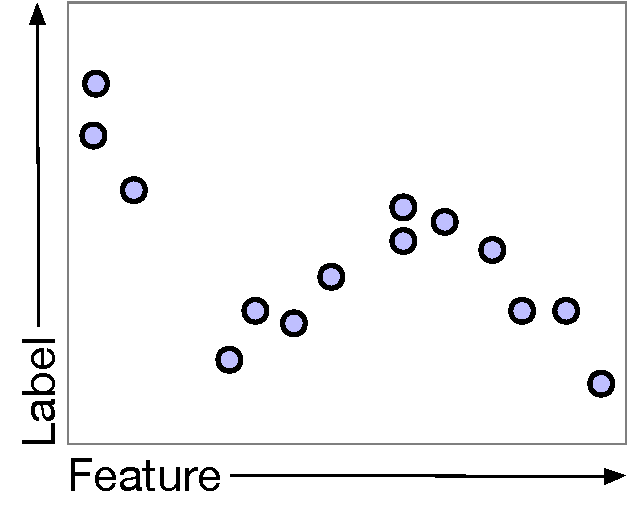
\includegraphics[width=.32\columnwidth]{img/classification-a}%
    \label{fig:classification-a}%
  }%
  \subfloat[][Fitted model]{%
    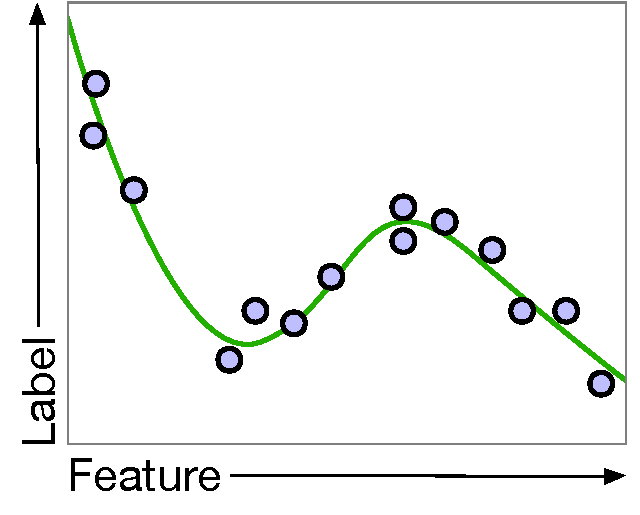
\includegraphics[width=.32\columnwidth]{img/classification-b}%
    \label{fig:classification-b}%
  }%
  \subfloat[][Model inference]{%
    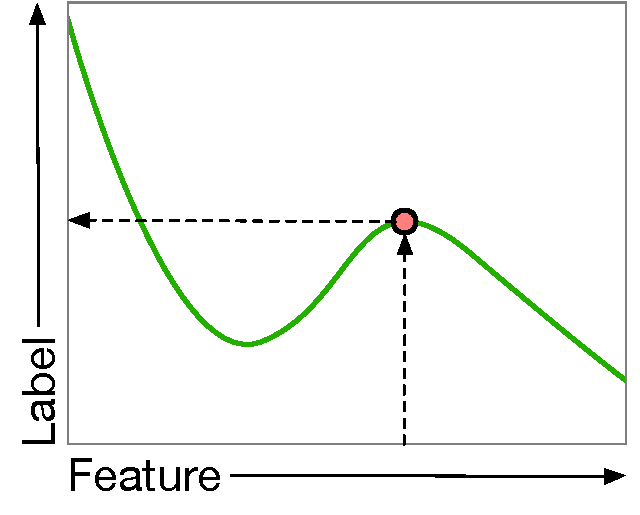
\includegraphics[width=.32\columnwidth]{img/classification-c}%
    \label{fig:classification-c}%
  }%
  \caption[Training and inference in machine learning]{%
    An illustration of the training and inference of a machine learning model. The $x$- and $y$-axes depict features and labels, which may be continuous or discrete multi-dimensional spaces. In~\subref{fig:classification-a}, training observations have been collected, consisting of features and their corresponding labels. A model is then fitted to these observations, shown as the green curve in~\subref{fig:classification-b}. The model can then be used to infer the label of unseen feature values, shown in~\subref{fig:classification-c}.%
  }%
  \label{fig:classification}
\end{figure}

Sequence modelling is the task of capturing the underlying probability distribution describing a sequence of values. This section describes the classification and sequential modelling techniques used in this thesis.


\subsection{Feed-forward Neural Networks}

Artificial Neural Networks comprise a network of artificial neurons and weighted connections between them to map input variables to a response. Figure~\ref{fig:artificial-neural-network} shows the architecture of a feed-forward artificial neural network. Each node represents an artificial neuron. The neurons are grouped into layers. The signal of an artificial neuron at a given layer is connected to the input of each artificial neuron in the next layer.

Intermediate layers for which there are no ground truth values are known as \emph{hidden} layers. Figure~\ref{fig:artificial-neural-network} depicts a three-layered network with three input values, a single hidden layer with four artificial neurons, and two outputs. Feed-forward multi-layered artificial neural networks are powerful \emph{universal function approximators}, capable of learning any bounded continuous function to arbitrary precision~\cite{Hornik1991,Lu2017,Yarotsky2017}.

\begin{figure}
  \centering
  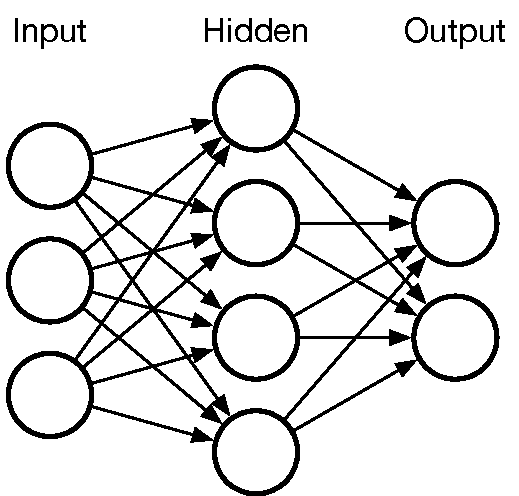
\includegraphics[width=.45\columnwidth]{img/artificial-neural-network}%
  \caption[Structure of an artificial neural network]{%
    A feed-forward artificial neural network with a single hidden layer. Each node in the graph depicts an artificial neuron, and each edge represents the output of one neuron connected to the input of another.%
  }%
  \label{fig:artificial-neural-network}
\end{figure}

The signal of an artificial neuron is the \emph{activation}. For a given layer $\ell$, the activations $\bm{a}^{[\ell]}$ are a function of the activations of the previous layer $\bm{a}^{[\ell - 1]}$, the connection weights $\bm{W}$, biases $\bm{b}$, and an activation function $\phi(z)$:

\begin{equation}
  \bm{a}^{[\ell]} = \phi \left( \bm{W}^{[\ell]^T} \bm{a}^{[\ell-1]} + \bm{b}^{[\ell]} \right)
\end{equation}

The connection weights and biases of an artificial neural network are adjusted during training such that, for a pair $(\bm{x}, y)$ where $\bm{x}$ is an input vector of features and $y$ is an observed label, the difference between the final layer activations and $y$ is minimised.


\paragraph*{Activation Function}

The activation function $\phi(z)$ is a non-linear differentiable function used to calculate the activation of an artificial neuron given a value $z \in \mathbb{R}$. A non-linear function is required to enable the ``stacking'' of artificial neuron layers to approximate non-linear functions. Commonly the \emph{Sigmoid} logistic function is used:

\begin{equation}
  \phi(z) = \frac{1}{1 + e^{-z}}
\end{equation}

Sigmoid activations are bounded in the range $(0,1)$, depicted in Figure~\ref{fig:activation-functions-sigmoid}.
% , which prevents blowing up of activations. Negative: gives rise to ``vanishing gradients'' because of the squishing behaviour for large positive or negative values - sigmoids saturate and kill gradients.
% It's output is not zero-centred, which makes gradient updates go too far in different directions.
For hidden layers, a disadvantage of sigmoid activation is that the output is not zero-centred. To address this, the \emph{Hyperbolic Tangent} (tanh) activation may be used, which is a scaled sigmoid function with values in the range $(-1,1)$:

\begin{equation}
  \phi(z) = \frac{e^{z} - e^{-z}}{e^z + e^{-z}}
\end{equation}

Figure~\ref{fig:activation-functions-tanh} illustrates the hyperbolic tangent activation. Logistic function-based activations suffer from a squashing effect with large positive and negative values, and they are \emph{dense} activations in which every artificial neuron contributes to the output value. The \emph{Rectified Linear Unit} (ReLU) activation function addresses both issues, with an unbounded range $[0,\infty)$:

\begin{equation}
  \phi(z) = max(z, 0)
\end{equation}

The ReLU activation is shown in Figure~\ref{fig:activation-functions-relu}. If initialised with random weights in the range $[-1,1]$, an average of 50\% of ReLU activated neurons will not fire, so that activations are sparse.
% Problem is ``dying'' neurons. When activations dip below 0, gradients will be 0, so the neuron becomes unresponsive to variations in input / error.
The \emph{Leaky ReLU} variation addresses the issue of large adjustments to parameters during training leading to neurons that are not activated for any input, effectively ``dying''. Leaky ReLU prevents artificial neurons from becoming unresponsive to variations in input by introducing a small slope for negative values:

\begin{align}
  \phi(z) =
    \begin{cases}
      0.01z, & \text{if } z < 0\\
      z, & \text{otherwise}
    \end{cases}
\end{align}

Typically a separate activation function is used for the output layer of an artificial neural network. For multi-class classification, \emph{softmax} may be used, which, for $K$ classes produces a vector:

\begin{equation}
  \phi(\bm{z})^{(i)} = \frac{e^{\bm{z}^{(i)}}}{\sum_{j=1}^{K} e^{\bm{z}^{(i)}}}, i = 1, \ldots, K
\end{equation}

Where $\sum_{i=1}^{K} \phi (\bm{z})^{(i)} = 1$.

\begin{figure}
	\centering
	% The empty square brackets are required to keep the (a), (b), and (c) subfloat labels.
	\subfloat[][Sigmoid]{%
		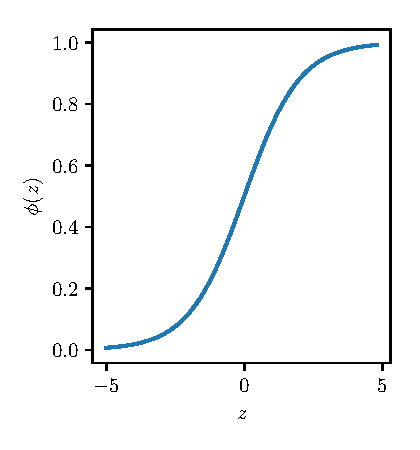
\includegraphics[width=.32\columnwidth]{img/activation-sigmoid}%
		\label{fig:activation-functions-sigmoid}%
	}%
	\subfloat[][Hyperbolic Tangent]{%
		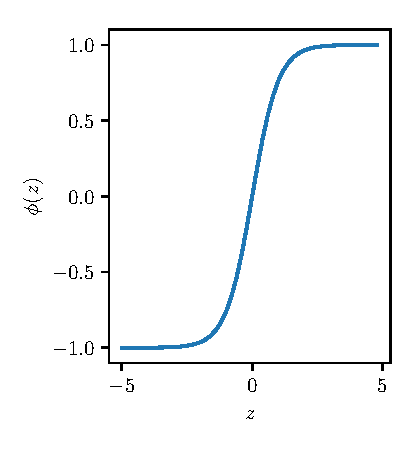
\includegraphics[width=.32\columnwidth]{img/activation-tanh}%
		\label{fig:activation-functions-tanh}%
	}%
	\subfloat[][Rectified Linear Unit]{%
		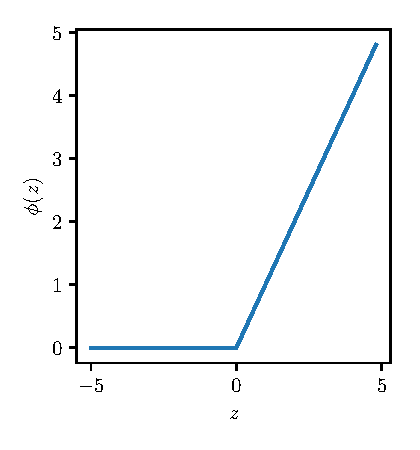
\includegraphics[width=.32\columnwidth]{img/activation-relu}%
		\label{fig:activation-functions-relu}%
	}%
	\caption[Activation functions for artificial neural networks]{%
      Three non-linear functions commonly used to determine the activation of artificial neurons in an artificial neural network.%
	}%
	\label{fig:activation-functions}
\end{figure}

\paragraph*{Backpropagation and Gradient Descent}

The most widely used technique to train artificial neural networks is backpropagation~\cite{Rumelhart1986}. Typically, the artificial neuron parameters are initialised with small random values. During training, a \emph{mini-batch} of $B$ observations is propagated through the network in a \emph{feed-forward} stage. The final outputs of the network $\bm{\hat{y}}$ are then compared against the true values $\bm{y}$ and used to compute an error $\mathcal{L}(\bm{\hat{y}}, \bm{y})$. The appropriate error function depends on the task. For a classification task with $K$ classes, \emph{categorical cross-entropy} may be used:

\begin{equation}
  \mathcal{L}(\bm{\hat{y}}, \bm{y}) = - \sum_{i=1}^K \bm{y}^{(i)} log (\bm{\hat{y}}^{(i)})
\end{equation}

For each layer $\ell$, the average error of the mini-batch $J$ is backpropagated through the network to update the connection weight $\bm{W}^{[\ell]}$ and bias parameters $\bm{b}^{[\ell]}$ based on a learning rate $\alpha$:

\begin{align}
J &= \frac{1}{B} \sum_{i=1}^B \mathcal{L}^{(i)}(\bm{\hat{y}^{(i)}}, \bm{y}^{(i)})\\
\bm{W}^{[\ell]} &= \bm{W}^{[\ell]} - \alpha \frac{\partial J}{\partial \bm{W}^{[\ell]}}\\
\bm{b}^{[\ell]} &= \bm{b}^{[\ell]} - \alpha \frac{\partial J}{\partial \bm{b}^{[\ell]}}
\end{align}

% TODO: Calculating derivatives through chain rule

% Where the derivative of the error function with respect to the network weights
%  derivative of sigmoid function $\phi(x)$:

% \begin{equation}
% \begin{aligned}
%   \phi(x) &= \frac{1}{1+e^{-x}}\\
%   \frac{\partial}{\partial x}\phi(x) &= \phi(x)(1 - \phi(x))
% \end{aligned}
% \end{equation}

\paragraph*{Regularisation Techniques}

Neural networks are vulnerable to \emph{over-fitting}, whereby the parameters of the model become specialised to the training observations, losing the ability to generalise to unseen data. Many \emph{regularisation} techniques have been adopted to mitigate the risk of over-fitting.

% Goodfellow, I., Bengio, Y., & Courville, A. (2016). Deep Learning. MIT PRess.
\emph{Dropout} is a regularisation technique in which a parameter in the range $[0,1]$ is used to determine a proportion of artificial neurons to be removed. This helps training by preventing complex co-adaptations on training values~\cite{Goodfellow2016}.



% \paragraph*{Normalization}

% Batch normalization


\subsection{Recurrent Neural Networks}

A Recurrent Neural Network (RNN)~\cite{Graves2012} is an artificial neural network in which the connections between artificial neurons form a cycle, enabling the processing of arbitrary size sequences by maintaining and updating a \emph{hidden state}.  RNNs are a \emph{deep learning} architecture, where deep learning is a loosely defined class of machine learning methods built on artificial neural networks\footnote{Deep learning is distinct from \emph{deep neural networks}, which are a specific deep learning architecture employing artificial neural networks with one or more hidden layers.}. Figure~\ref{fig:rnn} depicts an RNN, where $\bm{x}^{(t)} \in \mathbb{R}^d$ represents point $t \in \tau$ in a sequence of inputs $\bm{x} = \left( \bm{x}^{(1)}, \ldots, \bm{x}^{(\tau)} \right)$. The hidden states $\bm{h}^{(t)} \in \mathbb{R}^h$ and predicted output $\bm{\hat{y}}^{(t)} \in \mathbb{R}^y$ are updated at each step using:

\begin{figure}
  \centering
  % The empty square brackets are required to keep the (a) and (b) subfloat labels.
  \subfloat[][]{%
    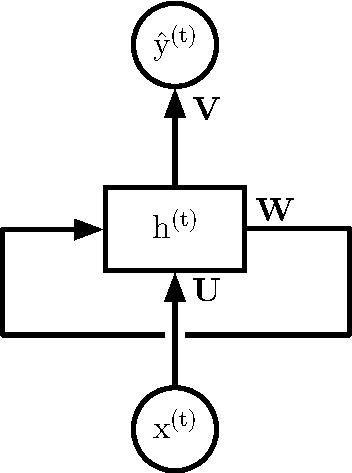
\includegraphics[height=5cm]{img/rnn-recurrence}%
    \label{fig:rnn-recurrence}%
  }%
  \hspace{1cm}
  \subfloat[][]{%
    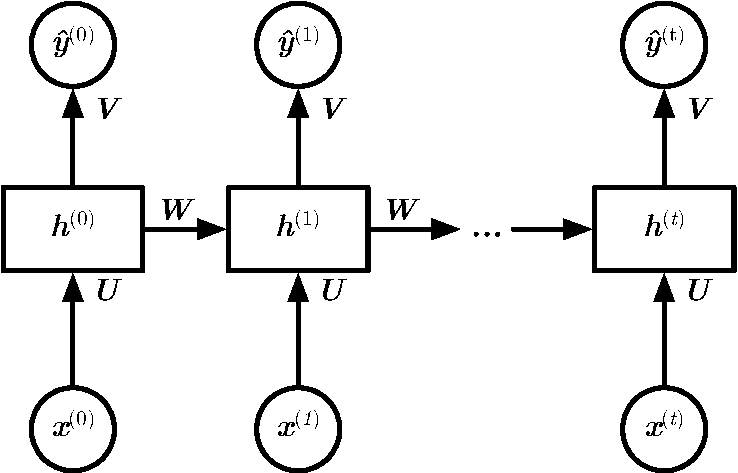
\includegraphics[height=5cm]{img/rnn-unrolled}%
    \label{fig:rnn-unrolled}%
  }%
  \caption[Recurrent Neural Network architecture]{%
    The computational graph of a Recurrent Neural Network, shown in~\protect\subref{fig:rnn-recurrence} as a recurrence relation, and unfolded in~\protect\subref{fig:rnn-unrolled}. $\bm{x}^{(t)}$ is the input, $\bm{h}^{(t)}$ is the hidden state, and $\bm{\hat{y}}^{(t)}$ is the output. The network is parameterised through three weight matrices: inputs-to-hidden weights $\bm{U}$, hidden-to-hidden weights $\bm{W}$, and hidden-to-output weights $\bm{V}$. As can be seen, the parameters are shared across all points in the time series.%
  }%
  \label{fig:rnn}
\end{figure}

\begin{align}
  \bm{h}^{(t)} &= \phi \left( \bm{U} \bm{x}^{(t)} + \bm{W} \bm{h}^{(t-1)} + \bm{b}_h \right) \\
  \bm{\hat{y}}^{(t)} &= \sigma \left( \bm{V} \bm{h}^{(t)} + \bm{b}_{\hat{y}} \right)
\end{align}

Where $\phi(\bm{z})$ and $\sigma(\bm{z})$ are non-linear activation functions, $\bm{b}_h$ and $\bm{b}_{\hat{y}}$ are bias vectors, and $\bm{W} \in \mathbb{R}^{h \times d}$, $\bm{U} \in \mathbb{R}^{h \times h}$, and $\bm{V} \in \mathbb{R}^{y \times h}$ are matrices representing the hidden-to-hidden, input-to-hidden, and hidden-to-output weights respectively.

The recurrent structure of RNNs enables the modelling of patterns in data with a temporal domain, such as text or numerical time series. Whereas a feed-forward artificial neural network estimates a conditional distribution based on an instantaneous input $p(y | \bm{x})$, an RNN estimates a distribution conditioned on $t$ prior observations $p\left(y^{(t)} | \{ \bm{x}^{(1)}, \ldots, \bm{x}^{(t)} \} \right)$.

Ordinary backpropagation may be used on an RNN by unfolding the computation graph over time, shown in Figure~\ref{fig:rnn-unrolled}. This \emph{backpropagation through time}~\cite{Werbos1990a} enables the propagation of errors in the temporal domain in the same manner as through layers.

% Siegelmann, H. T., & Sontag, E. D. (1991). Turing Computability with Neural Nets. Applied Mathematics Letters, 4(6).
RNNs are universal, in that any function computable by a Turing machine can be computed by an RNN of finite size~\cite{Sontag1991a}. In practice, a significant obstacle to the performance of RNNs is the diminishing ability to learn connections between values over long sequences. This is caused by the exponential diminishing and enlarging of gradients as they are propagated through non-linear activation functions by the recurrence relation. This issue is known as the
% Bengio, Y., Simard, P., & Frasconi, P. (1994). Learning Long-Term Dependencies with Gradient Descent is Difficult. IEEE Transactions on Neural Networks, 5(2).
\emph{vanishing gradients} problem~\cite{Bengio1994}.

% An RNN can learn a probability distribution over a sequence of tokens to predict the next token. Therefore, at each time step $t$, the output from the RNN conditional distribution $p\left( x_t | x_1, \ldots, x_{t-1} \right)$.

% De Boom, C., Dhoedt, B., & Demeester, T. (2018). Character-level Recurrent Neural Networks in Practice: Comparing Training and Sampling Schemes. ArXiv:1801.00632.
% \todo[inline]{RNN evaluation~\cite{DeBoom2018}.}


\paragraph*{Long Short-Term Memory}

Long short-term memory (LSTM)~\cite{Hochreiter1997} is an RNN architecture designed to overcome the vanishing gradients problem. The LSTM augments RNN design with the addition of a \emph{cell} for storing information, and three gates which control the flow of information into and out of the cell.

Figure~\ref{fig:lstm-block} depicts the structure of an LSTM cell. In addition to the recurrent connections for hidden states, a cell state vector $\bm{c}^{(t)} \in \mathbb{R}^h$ is propagated through time. The signal flow through the cell is controlled by three sigmoid activated gates: the forget gate $\bm{f}^{(t)} \in \mathbb{R}^h$, input gate $\bm{i}^{(t)} \in \mathbb{R}^h$, and output gate $\bm{o}^{(t)} \in \mathbb{R}^h$. At each time step, the values of the gate vectors are updated using:

\begin{figure}
  \centering
  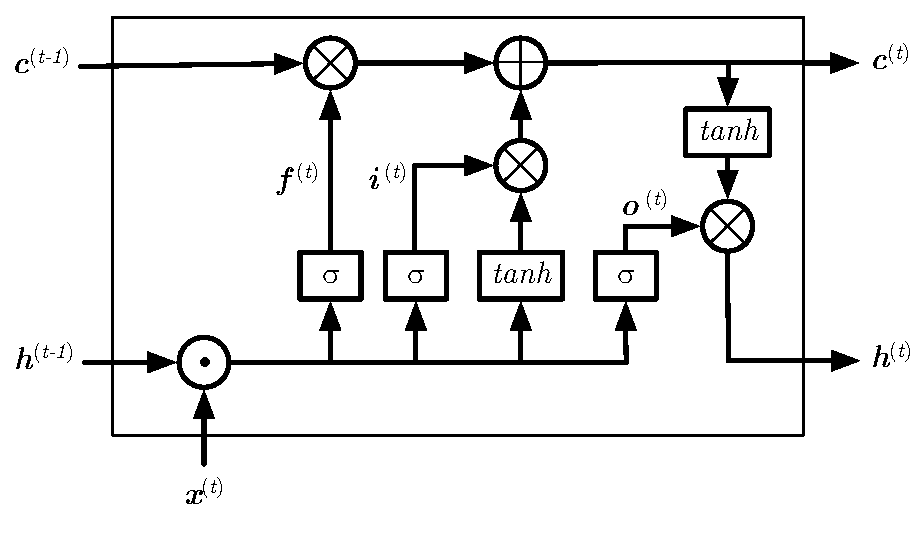
\includegraphics[width=.8\columnwidth]{img/lstm-block}%
  \caption[Long Short-Term Memory cell architecture]{%
    A Long Short-Term Memory cell block. Input $\bm{x}^{(t)}$ is concatenated with prior hidden state $\bm{h}^{(t-1)}$ and used along with prior cell state $\bm{c}^{(t-1)}$ to compute a new hidden state $\bm{h}^{(t)}$ and cell state $\bm{c}^{(t)}$. Symbols $\otimes$ denotes element-wise vector product, $\oplus$ element-wise vector addition, and $\odot$ vector concatenation.%
  }%
  \label{fig:lstm-block}
\end{figure}

\begin{align}
  \bm{f}^{(t)} &= \sigma \left( \bm{W}_f \bm{x}^{(t)} + \bm{U}_f \bm{h}^{(t-1)} + \bm{b}_f \right) \\
  \bm{i}^{(t)} &= \sigma \left( \bm{W}_i \bm{x}^{(t)} + \bm{U}_i \bm{h}^{(t-1)} + \bm{b}_i \right) \\
  \bm{o}^{(t)} &= \sigma \left( \bm{W}_o \bm{x}^{(t)} + \bm{U}_o \bm{h}^{(t-1)} + \bm{b}_o \right) \\
\end{align}

Where weight matrices $\bm{W} \in \mathbb{R}^{h\times d}$ and $\bm{U} \in \mathbb{R}^{h\times h}$, and bias vectors $\bm{b} \in \mathbb{R}^h$ are sub-scripted for the activation being calculated: $f$ forget gate, $i$ input gate, or $o$ output gate. The cell state and hidden state are then updated using:

\begin{align}
  \bm{c}^{(t)} &= \bm{f}^{(t)} \otimes \bm{c}^{(t-1)} + i^{(t)} \otimes tanh \left( \bm{W}_c \bm{x}^{(t)} + \bm{U}_c \bm{h}^{(t-1)} + \bm{b}_c \right) \\
  \bm{h}^{(t)} &= \bm{o}^{(t)} \otimes tanh ( \bm{c} ^{(t)} )
\end{align}

Where $\otimes$ denotes element-wise vector product, and subscript $c$ denotes cell state weight matrices and bias vectors. The gated cell enables LSTMs to build connections over long sequences in data. The LSTM architecture (and its many variants~\cite{Greff2015}) have been responsible for breakthrough results in a number of areas, for example machine translation~\cite{Sutskever2014}, speech recognition~\cite{Graves2005}, and weather prediction \cite{Shi2015a}.

% \subsection{Embedding}

\subsection{Decision Trees}

Decision trees are an intuitive form of classifier whereby a tree structure of decision nodes are used to predict the class for a given set of features. Decision trees are built using binary recursive partitioning: by creating an axis-parallel decision node for the feature which provides the highest gain, creating new child nodes for each possible outcome, splitting the data amongst these child nodes, and continuing recursively. The gain of a feature is found by first computing the entropy of the data set. Given a set of data points $D$ where $p_{(+)}$ is the number of positive examples in $D$ and $p_{(-)}$ is the number of negative examples in $D$:

\begin{equation}
  H(D) = - p_{(+)}\log_2p_{(+)} - p_{(-)}\log_2p_{(-)}
\end{equation}

The gain of a feature $x$ is found using:

\begin{equation}
  \gain(D, x) = H(D) - \sum_{V \in \text{Values}(x)}\frac{|D_V|}{|D|}H(D_V)
\end{equation}

Decision trees are a popular and low overhead form of classification. Once trained, a decision tree can be implemented as a set of nested conditional statements. This makes the learned model easily interpretable, simplifying debugging.

% TODO: \subsection{Generative Adversarial Networks}

% The Generative Adversarial Network (GAN) is a means to estimate a generative model~\cite{Goodfellow2014}. It uses an adversarial process in which two models are simultaneously trained: a generator model $G$ that captures the data distribution, and a discriminative model $D$ that estimates the probability that a sample came from the training data rather than $G$. The training procedure for $G$ is to maximise the probability of $D$ making a mistake.

% If both models are neural networks: learn a generator's distribution $p_g$ over data $\bm{x}$. Define a prior on input noise variables $p_z(\bm{z})$. Generator $G(\bm{z}; \Theta_g)$, using parameters $\Theta_g$. Discriminator $D(\bm{x}; \Theta_d)$ outputs a scalar, the probability that $\bm{x}$ came from the data rather than $p_g$.

% Simultaneously train $D$ to maximise the probability of assigning the correct label to both training examples and samples from $G$, and train $G$ to minimise $\log (1 - D(G(\bm{z})))$. $D$ and $G$ play the two-player minimax game with value function $V(G, D)$:

% \[ \min_G \max_D V(D, G) = \mathbb{E}_{\bm{x} \sim  p_{data}(\bm{x})} [ \log D(\bm{x}) ] + \mathbb{E}_{\bm{z} \sim p_z(\bm{z})} [ \log (1 - D(G(\bm{z}))) ] \]

% Challenge: there may not be sufficient gradient for $G$ to learn well. Early in learning, when $G$ is poor, $D$ can reject samples with high confidence because they are clearly different from the training data.



\section{Model Evaluation Techniques}
\label{sec:evaluation-techniques}

This section describes the techniques used to evaluate the machine learning methods described in the previous section.

\subsection{ZeroR}

A \emph{ZeroR} model is used in classification tasks to provide a baseline to evaluate the performance of classifiers. A ZeroR model represents the simplest approach to classification, its output is the mode of the training data labels, irrespective of the input. For example, given training data with the labels $\bm{y} = \{ A, B, B, C\}$, a ZeroR model will produce output $\bm{\hat{y}} = B$ for all future inputs. A ZeroR model has no power of prediction since its output is not conditioned on input features.


\subsection{Training, Validation, Test Data}

The data used to train a machine learning model must not be used to evaluate it. To evaluate a machine learning model, data must be divided into disjoint \emph{training} and \emph{testing} partitions. For a set of $N$ pairs of input and output observations $\bm{D} = (\bm{x}^{(i)}, \bm{y}^{(i)}), i = 1, \ldots, N$, let $k : {1,\ldots,N} \rightarrow {1,\ldots,K}$ be an indexing function that indicates the partition to which the observation $i \in N$ is allocated by the randomisation. The model is then trained with the $k$th part of the data removed, yielding fitted function $\hat{f}^{-k}(\bm{x})$. The quality of the model $V(\hat{f}^{-k})$ is then evaluated using the loss between the expected values and predicted values in the unseen test set:

\begin{align}
  \bm{y}_k &= \{ \bm{y}^{(i)} \in \bm{y} | i \in k(\bm{y}) \} \\
  V(\hat{f}^{-k}) &= \mathcal{L}(\bm{y}_k, \hat{f}^{-k}(\bm{x}_k))
\end{align}

Employing a second indexing function $u$ to divide the data not set aside for testing into disjoint \emph{training} and \emph{test} sets creates a \emph{validation} set. A validation set can be used to automatically tune model parameters. Given a model $f_p$ parameterised by $p$, the quality of the model evaluating using the parameters $\bar{p}$ that provide the smallest loss on the validation set can be found from a set of parameters $P$ using:

\begin{align}
  \bar{p} &= \argmin_p \mathcal{L}(\bm{y}_u, \hat{f}_p^{-(k \cup u)}(\bm{x}_u)), \hspace{.5em} p \forall P\\
  V(\hat{f}_{\bar{p}}^{-k}) &= \mathcal{L}(\bm{y}_k, \hat{f}_{\bar{p}}^{-(k \cup u)}(\bm{x}_k))
\end{align}

\subsection{$K$-Fold Cross-validation}

Dividing the dataset into fixed training and test sets is problematic if it results in the test set being small. A small test set implies statistical uncertainty around the estimated average test error, making it difficult to compare models.

Ideally, sufficient data would exist to be set aside for testing. When not practically possible, cross-validation may be used. Cross-validations enables the use of all observations in a data set in the estimation of the mean test error, at the expense of increased computational cost through repeated evaluations.

K-Fold cross-validation sets aside part of the available data to fit the model, and a different part to test it. Data is split into $K$ roughly equal-sized parts.

\begin{equation}
  CV(\hat{f}) = \frac{1}{K}\sum_{i=1}^K \mathcal{L}(\bm{y}^{(i)}, \hat{f}^{-K^{(i)}}(\bm{x}^{(i)}))
\end{equation}

Where for a set of $n$ observations, $K \le n$. If $K=n$ this is known as \emph{leave-one-out} cross-validation.

For a classification task, if observations are distributed amongst the $K$ partitions such that the distribution of observed classes in all partitions is equal, this is called \emph{stratified} $K$-fold cross-validation.


\subsection{Principal Component Analysis}

Principal Components Analysis PCA~\cite{Jolliffe2011} is a statistical procedure for identifying the underlying components responsible for variance in data. Given $n$ dimensions of observations, PCA produces a $k$-dimensional subspace through a linear transformation, where $k < n$. Each component is ordered by decreasing variance, $Var(k^{(i)}) \le Var(k^{(i-1)})$. This dimensionality-reduction is useful for exposing underlying correlations in machine learning feature design, and to aid in visually inspecting high-dimensional spaces where $n \ge 3$.

To compute the principal components, one begins with a normalised matrix of observations $\bm{X} \in \mathbb{R}^{m \times n}$ of $m$ rows and $n$ columns (components). The data is normalised to the range $[-1,1]$ by subtracting the mean and scaling each component by its variance. Given eigenvectors $\bm{v}^{(1)}, \ldots \bm{v}^{(m)}$, the matrix of $k$ principal components $\bm{\hat{X}} \in \mathbb{R}^{m \times k}$ can be computed using:

\begin{equation}
\bm{\hat{X}} = [ \bm{v}^{(1)}, \ldots, \bm{v}^{(k)}]^T \cdot \bm{X}\\
\end{equation}

% \section{Heterogeneous Systems}
% \label{sec:programming-heterogeneous-systems}

% A heterogeneous system contains multiple types of processor. Compared to systems with a single processor, programming for heterogeneous systems is especially challenging. Typical approaches divide the system processors into a \emph{host processor} and one or more additional \emph{accelerator} processors, where the host processor is responsible for coordinating and synchronising work on the accelerator processors. This approach has been successfully used for General-purpose computing on Graphics Processing Units (GPGPU), where the system CPU is the host and the GPUs are used as accelerators~\cite{Owens2006}. Many of the techniques in this thesis are evaluated using OpenCL, a popular language and framework for programming heterogeneous systems.


% \subsection{OpenCL Programming Model}

% OpenCL is a vendor-independent open standard for programming heterogeneous systems, supporting CPUs, GPUs, and other parallel processors such as Field-Programmable Gate Arrays~\cite{Stone2010}. It comprises a compute language based on a subset of the ISO C99 programming language, and a suite of APIs for controlling heterogeneous compute devices from a central host. Programs written for these devices are called kernels, and are compiled by platform-specific toolchains. At runtime, an OpenCL platform is selected and a context object is created which exposes access to each supported compute device through command queues. When a kernel is executed, each unit of computation is referred to as a work-item, and these work-items are grouped into work-groups. The sum of all work-group dimensions defines the global size. For GPUs, work-groups execute on the Single Instruction Multiple Data (SIMD) processing units in lock-step. This is different from the behaviour of traditional CPUs, and can cause severe performance penalties in the presence of flow control, as work-items must be stalled across diverging flow paths.


% % \paragraph*{Memory Model}

% OpenCL uses a hierarchical memory model, shown in Figure~\ref{fig:opencl-memory-hierarchy}. The host and each OpenCL device has a single global memory address space. Each work-group has a local memory space, and each work-item has a region of private memory.

% \begin{figure}
%   \centering
%   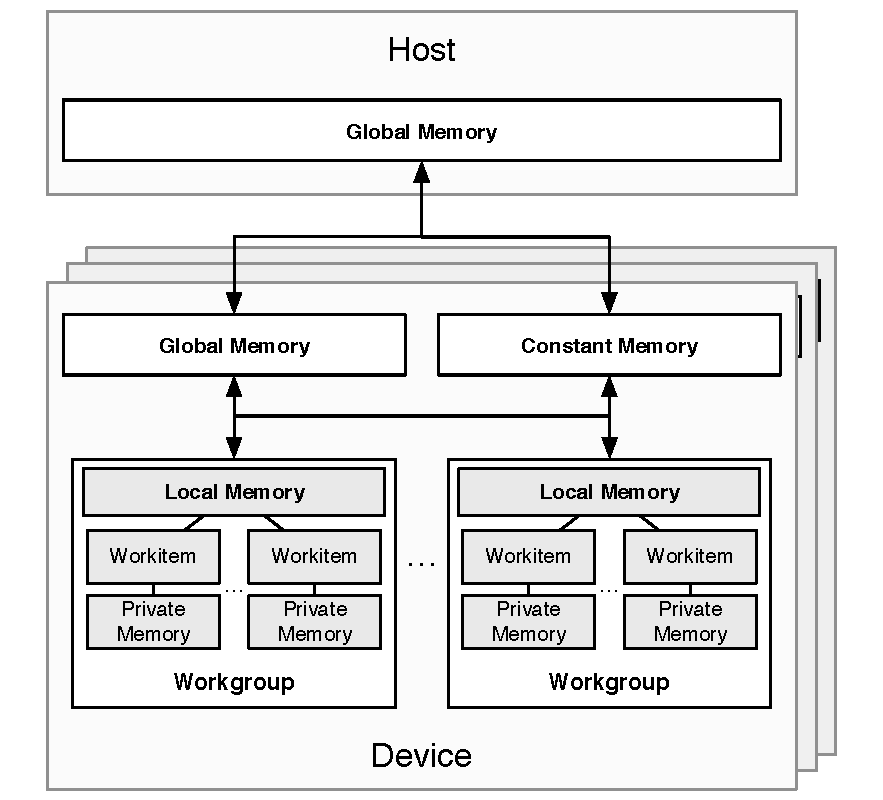
\includegraphics[width=0.8\textwidth]{img/opencl-memory}
%   \caption[OpenCL memory model]{%
%     The OpenCL memory model. The host communicates with each device through transfers between global memory spaces. The capacity of each type of memory is dependent on the device hardware. In general, private memory is the fastest and smallest, and global memory is the largest and slowest.%
%   }
%   \label{fig:opencl-memory-hierarchy}
% \end{figure}

% Work-groups cannot access the memory of neighbouring work-groups, nor can work-items access the private memory of other work-items. OpenCL provides synchronisation barriers to allow for communication between work-items within a single work-group via the local memory, but not global barriers. Memory transfers between the host and devices occurs between global memory regions. In the case of programming heterogeneous devices, these transfers must occur over the connection bus between the CPU and device (e.g.\ PCIe for discrete GPUs), which typically creates a performance bottleneck by introducing a performance overhead to transfer data to the device for processing, then back to the device afterwards.


% \subsubsection{Performance Optimisations}

% Optimising OpenCL is challenging because of the wide range of supported execution devices. Performance portability is challenging because each standards-compliant implementation differs~\cite{Rul2010}, and the interactions between optimisations and the hardware are complex and sometimes counter-intuitive~\cite{Ryoo2008}.

% The overhead introduced by memory transfers between host and compute devices further complicates comparisons of OpenCL performance on different devices. The conclusion of~\cite{Gregg2011} is that this overhead can account for a $2\times$ to $50\times$ difference of accelerator program runtime. In~\cite{Lee2010}, \citeauthor{Lee2010} present a performance analysis of optimised throughput computing applications for GPUs and CPUs. Of the 14 applications tested, they found GPU performance to be $0.7\times$ to $14.9\times$ that of multi-threaded CPU code, with an average of only 2.5$\times$. This is much lower than the $100\times$ to $1000\times$ values reported by other studies, a fact that they attribute to uneven comparison of optimised GPU code to unoptimised CPU code, or vice versa. \citeauthor{Lee2010} found that multi-threading, cache blocking, reordering of memory accesses and use of SIMD instructions to contribute most to CPU performance. For GPUs, the most effective optimisations are reducing synchronisation costs, and exploiting local shared memory. In all cases, the programs were optimised and hand-tuned by programmers with expert knowledge of the target architectures. It is unclear whether their performance results still hold for subsequent generations of devices.

% Despite the concerns of over-represented speedups, the potential for high performance coupled with the complexity and low-levels of abstraction provided by OpenCL make it an ideal target for skeletal abstractions. SkelCL and SkePU are two such examples which add a layer of abstraction above OpenCL and CUDA respectively in order to simplify GPGPU programming~\cite{Enmyren2010}.


% \subsection{Evaluation Techniques}
% \label{subsec:background-statistics}

% This section describes a number of the statistical tools and evaluation techniques used throughout this thesis.


% \subsubsection{Interquartile Range}

% Quartiles are the three points that divide an ordered set of data values into four groups of equal size. The first quartile $Q_1$ is the point which divides the data equally between the lowest value and the median, $Q_2$. The third quartile $Q_3$ is the point which divides the data between the median and the highest value. The interquartile range (IQR) measures the dispersion of a data set, and is the difference between the third and first quartiles, $Q_3 - Q_1$.


% \subsubsection{Confidence Intervals}

% Confidence intervals estimate the interval for the true range of a population parameter. Given a set of samples of a population with estimates of a parameter value for each, the confidence interval $(c_1,c_2)$ estimates the frequency that the true parameter value will fall between the per-sample confidence interval. Given a sample $x$ with sample size $n$, the confidence interval for a confidence $\alpha$ is found using:

% \begin{align}
%   \bar{x} &= \frac{1}{n}\sum_{i=1}^{n} x_i\\
%   \sigma &= \sqrt{\frac{\sum_{i=1}^{n}(x_i - \bar{x})^2}{n - 1}}\\
%   c_1 &= \bar{x} - z_{1-\alpha/2}\frac{\sigma}{\sqrt{n}}\\
%   c_2 &= \bar{x} + z_{1-\alpha/2}\frac{\sigma}{\sqrt{n}}
% \end{align}

% Where the value $z_{1-\alpha/2}$ assumes a Gaussian distribution of
% the underlying data, and the values for popular $\alpha$ values are
% typically found using pre-computed ``Z-tables''. To calculate
% confidence intervals for the ratio of two means, $\bar{x}_1$ and
% $\bar{x}_2$ with sample sizes $n_1$ and $n_2$, and respective standard
% deviations $\sigma_1$ and $\sigma_2$:

% \begin{align}
%   \sigma_x &= \sqrt{\frac{\sigma_1^2}{n_1} + \frac{\sigma_2^2}{n_2}}\\
%   c_1 &= \bar{x}_1 - \bar{x}_2 - z_{1-\alpha/2}\sigma_x\\
%   c_2 &= \bar{x}_1 - \bar{x}_2 + z_{1-\alpha/2}\sigma_x
% \end{align}

% The above calculations assumes that the sample variance ($\sigma^2$)
% is an accurate estimation of the true population variance. This relies
% on the assumption of an underlying Gaussian distribution, which,
% according to the central limit theorem, is true of large sample sizes
% (typically $n \ge 30$). In cases of smaller sample sizes, the sample
% and population variances can differ significantly, so one must instead
% use a Student's $t$-distribution, $t_{1-\alpha/2}$, in place of
% $z_{1-\alpha/2}$.


% \subsubsection{Histogram}

% Histograms show the distribution of numerical data. The data is first divided into a set of discrete, equally sized sub-intervals, or \emph{bins}. The number of data points in each bin is used to show visualise the density distribution. The shortcoming of histograms is that their appearance is heavily influenced by three user-selected parameters: the number of bins, the width of bins, and the endpoints chosen. As such, they may provide a misleading representation of the data if inappropriate values for any of these parameters are chosen. Kernel Density estimation is a technique for showing the distribution of data which circumvents some of these issues.

% \subsubsection{Kernel Density Estimation}

% A Kernel Density Estimate (KDE) is an approximation of the probability
% density function of a random variable. Given a random variable $x$,
% and bandwidth $h$ and a kernel $K$, the Kernel Density Estimate
% $\hat{f}_h(x)$ can be found using:
% %
% \begin{equation}
%   \hat{f}_h(x) = \frac{1}{nh} \sum^{n}_{i=1} K\left( \frac{x - x_i}{h} \right)
% \end{equation}
% %
% Using a smooth kernel such as a Gaussian distribution for the kernel
% produces a smooth density estimated, unlike histograms. However, like
% histograms, the appearance of a Kernel Density Estimate plot is
% dependent on the value of the bandwidth parameter $h$ (equivalent to
% binwidth in histograms), so care must be taken to select a value to
% minimise over or under smoothing. Grouped data can be shown by
% plotting multiple KDEs on the same axes, although if the number of
% groups is large, a box plot or violin plot may be more appropriate.


% \subsubsection{Box plot}

% Box plots are used to show the distribution of quartile ranges for
% grouped data. The contain the following features:
% %
% \begin{itemize}
%   \item Horizontal lines at the lower quartile, median and upper
%   quartile.
%   \item Vertical lines above and below the upper and lower quartiles to
%   the most extreme data point within 1.5 IQR of the upper/lower
%   quartile, with horizontal whiskers at the end of the vertical lines.
%   \item Dots beyond the ends of the vertical lines to show outliers.
% \end{itemize}
% %
% A variation of box plots used in this thesis is the violin plot, which
% extends the box plot with a fitted Kernel Density Estimate plot to
% show the probability \emph{density} of data at different values. To
% construct a violin plot, KDEs for each group are rotated and mirrored
% to generate a smoothed visualisation of the distribution.



% \section{Differential Testing}

% \todo[inline]{Difftesting overview, including the figure from the litreview.}


\section{Summary}
\label{sec:background-summary}

This chapter provides background on the machine learning techniques used in this thesis to develop low cost techniques for compiler construction, and the techniques used in evaluating their effectiveness. The following chapter surveys research literature relevant to this work.
